\section{General Bipartite Graphs}
\label{sec:general}
In this section, we will show how the NP-completeness result in star graphs results in NP-hardness of recognizing core imputations of general bipartite graphs. We will also show that this, in turn, translates to the NP-hardness of recognizing if an imputation is the leximin(or leximax) core imputation.  
% \todo {talk about leximin and leximax}

\subsection{Core imputations}

\begin{theorem}
\label{thm:core_coNP_complete}
    Deciding if an imputation is in the core of $b$-matching games on general bipartite graphs is co-NP-Complete.
\end{theorem}
% \todo {how can we handle the long proof of this theorem?}


% \begin{theorem}
%     There's a pseudo-polynomial time algorithm to check if a profit share is in the core of $b$-matching games on general bipartite graphs graphs.
% \end{theorem}

\begin{proof}
Clearly, the problem lies in co-NP, since a co-NP certificate for this problem would be a sub-coalition which is not satisfied under the imputation.\\ 
We will prove that deciding if an imputation is in the core of a bipartite $b$-matching game is co-NP-hard. In this regard, we use a reduction from the problem in~\Cref{thm:profit_share_for_star}. We will construct a bipartite graph $G'$ by adding 2 vertices to a star graph $G$ such that, there is an unstable sub-coalition of agents $S$ in $G'$ if and only if $S$ is an unstable coalition in $G$.

%We aim to transform the star graph of Lemma 1 into a graph $ G $ such that determining whether an imputation belongs to the core of $ G $ reduces to deciding whether a semi-imputation belongs to the semi-core of the original star graph. Specifically, we will add vertices $ x $ and $ y $ to the star graph, ensuring that any unstable coalitions of the resulting graph $ G $ correspond to unstable coalitions of the original star graph.

\begin{figure}[H]
    \centering
    \begin{minipage}{0.48\textwidth}
        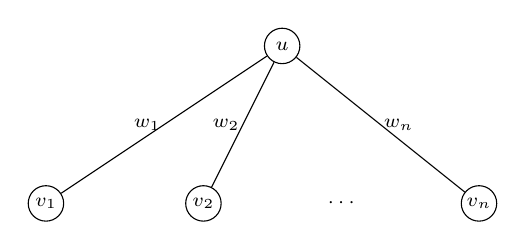
\begin{tikzpicture}[scale=1, every node/.style={inner sep=1pt}]
            \scriptsize
            % Nodes
            \node[draw, circle, minimum size=0.45cm] (u) at (0, 2) {$u$};
            \node[draw, circle, minimum size=0.45cm] (v1) at (-3, 0) {$v_1$};
            \node[draw, circle, minimum size=0.45cm] (v2) at (-1, 0) {$v_2$};
            \node[draw, circle, minimum size=0.45cm] (vn) at (2.5, 0) {$v_n$};

            % Connecting edges
            \draw (u) -- (v1) node[midway, left] {$w_1$};
            \draw (u) -- (v2) node[midway, left] {$w_2$};
            \draw (u) -- (vn) node[midway, right] {$w_n$};
            % Dots
            \path (v2) -- (vn) node[midway, draw=none] {$\cdots$};
        \end{tikzpicture}
    \end{minipage}
    \hfill
    \begin{minipage}{0.48\textwidth}
        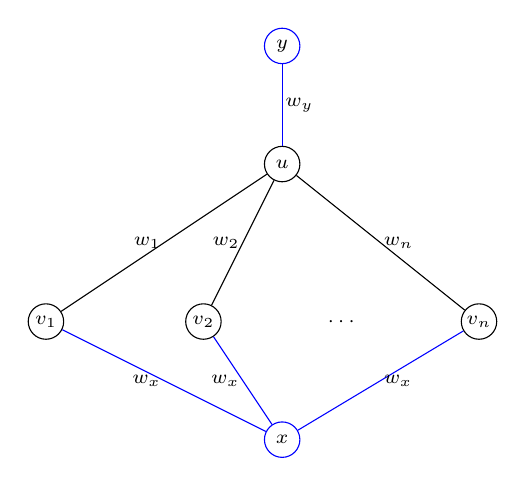
\begin{tikzpicture}[scale=1, every node/.style={inner sep=1pt}]
            \scriptsize
            % Nodes
            \node[draw, circle, minimum size=0.45cm] (u) at (0, 2) {$u$};
            \node[draw=blue, circle, minimum size=0.45cm] (y) at (0, 3.5) {$y$};
            \node[draw, circle, minimum size=0.45cm] (v1) at (-3, 0) {$v_1$};
            \node[draw, circle, minimum size=0.45cm] (v2) at (-1, 0) {$v_2$};
            \node[draw, circle, minimum size=0.45cm] (vn) at (2.5, 0) {$v_n$};
            \node[draw=blue, circle, minimum size=0.45cm] (x) at (0, -1.5) {$x$};

            % Connecting edges
            \draw (u) -- (v1) node[midway, left] {$w_1$};
            \draw (u) -- (v2) node[midway, left] {$w_2$};
            \draw (u) -- (vn) node[midway, right] {$w_n$};
            \draw[draw=blue] (u) -- (y) node[midway, right] {$w_y$};
            \draw[draw=blue] (v1) -- (x) node[midway, left] {$w_x$};
            \draw[draw=blue] (v2) -- (x) node[midway, left] {$w_x$};
            \draw[draw=blue] (vn) -- (x) node[midway, right] {$w_x$};

            % Dots
            \path (v2) -- (vn) node[midway, draw=none] {$\cdots$};
        \end{tikzpicture}
    \end{minipage}
    \caption{(Left) $G^*;\quad\quad$(Right) Add blue vertices and edges to $G^*$ to get $G$  }
    \label{fig:side_by_side_graph}
\end{figure}

%  \begin{center}
%     \begin{tikzpicture}[scale=1.5, every node/.style={inner sep=1pt}]
%         \small
%         % Nodes
%         \node[draw, circle, minimum size=0.45cm] (u) at (0, 2) {$u$};
%         \node[draw=blue, circle, minimum size=0.45cm] (y) at (0, 3.5) {$y$};
%         \node[draw, circle, minimum size=0.45cm] (v1) at (-3, 0) {$v_1$};
%         \node[draw, circle, minimum size=0.45cm] (v2) at (-1, 0) {$v_2$};
%         \node[draw, circle, minimum size=0.45cm] (vn) at (2.5, 0) {$v_n$};
%         \node[draw=blue, circle, minimum size=0.45cm] (x) at (0, -1.5) {$x$};

        
%         % Connecting edges
%         \draw (u) -- (v1) node[midway, left] {$w_1$};
%         \draw (u) -- (v2) node[midway, left] {$w_2$};
%         \draw (u) -- (vn) node[midway, right] {$w_n$};
%         \draw[draw=blue] (u) -- (y) node[midway, right] {$w_y$};
%         \draw[draw=blue] (v1) -- (x) node[midway, left] {$w_x$};
%         \draw[draw=blue] (v2) -- (x) node[midway, left] {$w_x$};
%         \draw[draw=blue] (vn) -- (x) node[midway, right] {$w_x$};

      
%         % Dots
%         \path (v2) -- (vn) node[midway, draw=none] {$\cdots$};
%     \end{tikzpicture}
% \end{center}
% \begin{center}
%     \begin{tikzpicture}[scale=1.5, every node/.style={inner sep=1pt}]

% % Nodes
% \node[draw, circle, minimum size=0.6cm] (u) at (0, 2) {$u$};
% \node[draw, circle, minimum size=0.6cm] (y) at (0, 3.5) {$y$};
% \node[draw, circle, minimum size=0.6cm] (v1) at (-2, 0) {$v_1$};
% \node[draw, circle, minimum size=0.6cm] (v2) at (-1, 0) {$v_2$};
% \node[draw, circle, minimum size=0.6cm] (vn) at (2, 0) {$v_n$};
% \node[draw, circle, minimum size=0.6cm] (x) at (0, -1.5) {$x$};

% % Connecting edges
% \draw (u) -- (v1) node[midway, left] {$w_1$};
% \draw (u) -- (v2) node[midway, left] {$w_2$};
% \draw (u) -- (vn) node[midway, right] {$w_n$};
% \draw (u) -- (y) node[midway, right] {$w_y$};
% %\draw[bend left] (y) to node[midway, above] {$w_y$} (u);
% \draw (v1) -- (x) node[midway, left] {$w_x$};
% \draw (v2) -- (x) node[midway, left] {$w_x$};
% \draw (vn) -- (x) node[midway, right] {$w_x$};

% % Dots
% \path (v2) -- (vn) node[midway, draw=none] {$\cdots$};

% \end{tikzpicture}
% \end{center}

To construct $ G=(U,V,E) $ consider same graph $G^*=(U^*,V^*,E^*)$ of~\Cref{thm:profit_share_for_star} and we add two vertices $x$ and $y$ as follows:
\begin{itemize}
    \item vertex $ x $ is connected to all $ v_i $ with edges of weight $ w_x $.
    \item vertex $ y $ is connected to $ u $ with an edge of weight $ w_y $.
\end{itemize}
%\todo{define $G'$ better}
So we have $G=(U,V,E)$ such that $U=U^* \cup\{x\}$, $V=V^*\cup\{y\}$, $E=E^*\cup\{(y,u),(x,v_1),$ $(x,v_2),\dots,(x,v_n)\}$

The parameters of the graph are defined as follows:
$$
w_x = \sum_{i=1}^n p_i + 1, \quad w_y = p_u + 1,
$$
$$
b_x = \sum_{i=1}^n b_i, \quad b_y = b_u,
$$
$$
p_x = (b_x - 1)w_x + 1, \quad p_y = (b_y - 1)w_y + 1.
$$


Firstly, we show that $p$ is an imputation in $G$, i.e., we need to show that $p(G) = \nu(G)$. So let us compute these values.

\begin{claim}
    $$p(G) = b_xw_x + b_yw_y$$
\end{claim}

\begin{proof}
The profit $ p(G) $ is the sum of profits assigned to all vertices:
    \begin{align*}
p(G) & = p_x + p_y + p_u + \sum_{i=1}^n p_i.\\
& = (b_x - 1)w_x + 1 + (b_y - 1)w_y + 1 + p_u + \sum_{i=1}^n p_i.\\
 &= b_x w_x - w_x + 1 + b_y w_y - w_y + 1 + p_u + \sum_{i=1}^n p_i\\
 &= b_x w_x - \left( \sum_{i=1}^n p_i + 1 \right) + 1 + b_y w_y - (p_u + 1) + 1 + p_u + \sum_{i=1}^n p_i.\\
\Rightarrow p(G) &= b_x w_x + b_y w_y.
\end{align*}
\end{proof}

% \subsection*{Computing $ p(G') $}
% \todo{Should we remove this part? I wrote it as a claim}
% The profit $ p(G') $ is the sum of profits assigned to all vertices:
% $
% p(G') = p_x + p_y + p_u + \sum_{i=1}^n p_i.
% $
% Substituting the definitions:
% $
% p(G') = (b_x - 1)w_x + 1 + (b_y - 1)w_y + 1 + p_u + \sum_{i=1}^n p_i.
% $
% Simplifying:
% $
% p(G') = b_x w_x - w_x + 1 + b_y w_y - w_y + 1 + p_u + \sum_{i=1}^n p_i.
% $
% Expanding $ w_x $ and $ w_y $:
% $
% p(G') = b_x w_x - \left( \sum_{i=1}^n p_i + 1 \right) + 1 + b_y w_y - (p_u + 1) + 1 + p_u + \sum_{i=1}^n p_i.
% $
% This simplifies to:
% $
% p(G') = b_x w_x + b_y w_y.
% $
\begin{claim}
    $$\nu(G') = b_xw_x+b_yw_y$$
\end{claim}
\begin{proof}
    The value $ \nu(G) $ is the max. wt. $ b $-matching in the graph $ G $. First, we show that in the max. wt. $ b $-matching of $ G $, no edge of the form $ (u,v_i) $ is used.
 
Suppose an edge $ (u,v_i) $ is included in the max. wt. $ b $-matching. We can remove this edge and instead add the edges $ (x,v_i) $ and $ (y,u) $. The value of the game then decreases by $ w_i $, from removing $ (u,v_i) $, but increases by $ w_x + w_y $, from adding $ (x,v_i) $ and $ (y,u) $). Since,
$$
w_x + w_y = \left( \sum_{i=1}^n p_i + 1 \right) + \left( p_u + 1 \right) = p(G) + 2,
$$
and $ p(G) + 2 > w_i $, this contradicts the maximality of the $ b $-matching.

Hence, no edges of the form $ (u,v_i) $ are used in the max. wt. $ b $-matching. Therefore, we can choose all edges adjacent to $x$ and $y$ upto their full capacities, without exceeding the capacities of other vertices to get the max. wt. $b$-matching. Hence, 
$
\nu(G') = b_x w_x + b_y w_y.
$
\end{proof}
\begin{corollary}
    $p(G) = \nu(G)$ so $p$ is an imputation for $G$.
\end{corollary}
% \subsection*{Computing $ \nu(G') $}
% \todo{Should we remove this part? I write it as a claim}
% The value $ \nu(G') $ is the max. wt. $ b $-matching in the graph $ G' $. First, we show that in the max. wt. $ b $-matching of $ G' $, no edge of the form $ uv_i $ is used.

% \textbf{proof by contradiction:}  
% Suppose an edge $ uv_i $ is included in the max. wt. $ b $-matching. We can remove this edge and instead add the edges $ xv_i $ and $ yu $. The value of the game then decreases by $ w_i $ (from removing $ uv_i $) but increases by $ w_x + w_y $ (from adding $ xv_i $ and $ yu $). Since:
% $
% w_x + w_y = \left( \sum_{i=1}^n p_i + 1 \right) + \left( p_u + 1 \right) = p(G') + 2,
% $
% and $ p(G') + 2 > w_i $, this contradicts the maximality of the $ b $-matching.

% Hence, no edges of the form $ uv_i $ are used in the max. wt. $ b $-matching. Therefore:
% $
% \nu(G') = b_x w_x + b_y w_y.
% $

% From the above, we conclude:
% $
% p(G') = \nu(G').
% $

%Now, we want to prove that if there is an unstable coalition such $S$ ($p(S) < \nu(S)$) then $S \cap \{x,y\} = \emptyset $. In this regard, we first prove a similar property as lemma \ref{fully matched in star}.

\begin{lemma}
    Let $S$ be an unstable coalition containing $x$ or $y$ which are not fully matched in any max. wt. $b$-matching in $S$. Then $S\setminus \{x,y\}$ is also an unstable coalition. 
  % Let $S \subseteq U\cup V$ such that $\nu(S) > p(S)$. If there exists a vertex $v \in \{x,y\}$ and $v\in S$ and $v$ is not fully matched in the max. wt. $b$-matching of $S$ then:
  % $$\nu(S \backslash\{v\}) > p(S\backslash\{v\})$$
\end{lemma}

\begin{proof}
Let us consider both cases. \\
\begin{itemize}
\vspace{-6mm}
    \item[] \textbf{Case(\textit{i}): }$v = x$ : 

        Removing $ x $ decreases the profit by $ p_x $ and as $x$ is not fully matched, the value is decreased by at most $ (b_x - 1)w_x $ Thus, $\nu(S) - p(S) \text{ increases by at least } p_x - (b_x - 1)w_x$.

    \item[]\textbf{Case(\textit{ii}): $v = y$} : 
        
        By a similar argument as above we can say that by removing $v_y$, $\nu(S) - p(S)$ increases by at least $ p_y - (b_y - 1)w_y$.
        
\end{itemize}
       
    As we have $p_x - (b_x - 1)w_x = p_y - (b_y - 1)w_y = 1 $, in both cases $\nu(S \backslash\{v\}) - p(S\backslash\{v\}) > \nu(S) - p(S)$. So if $S$ is an unstable coalition that does not fully match $x$ or $y$, then $S\setminus{\{x,y\}}$ is also an unstable coalition. 
\end{proof}

\begin{observation}
    If $S$ is a sub-coalition that maximizes $\nu(S) - p(S)$ and contains $x$ or $y$, then they must be fully matched in every max. wt. $b$-matching of $S$.
    % There is a subset of vertices $S$ which maximizes $\nu(S) - p(S)$ such that if $x$ or $y$ is in it they have to be fully matched in the max. wt. $b$-matching of $S$
\end{observation}
\begin{claim}
    No unstable coalition in $G$ contains $x$ or $y$.
    % If there is a unstable coalition such $S$ ($p(S) < \nu(S)$) then $S \cap \{x,y\} = \emptyset $.
\end{claim}
\begin{proof}

Consider a set $ S $ that maximizes $ \nu(S) - p(S) $. If both $ x $ and $ y $ are in $ S $, they must be fully matched, which implies that all vertices should be included in $ S $. Hence, $ S = G $, and we obtain $ \nu(S) - p(S) = 0 $.

Now, consider the case where $ y $ is in $ S $ but $ x $ is not. Since $ y $ must be fully matched, the edge $ (u,y) $ is chosen to satisfy the capacity of $ u $. Consequently, no edge $ (u,v_i) $ can be matched. Because $ x $ is not in $ S $, the presence of any $ v_i $ does not increase the value of $ S $, and thus these vertices can be removed to maximize $ \nu(S) - p(S) $. Removing all such vertices, we obtain $ S = \{y,u\} $. However, this is not an unstable coalition, as shown by the following computation:
$$p(S) = p_y + p_u = (b_y - 1)w_y + 1 + p_u = (b_u - 1)(p_u + 1) + p_u = b_up_u + b_u $$
$$\nu(S) = b_y.w_y = b_u(p_u+1) = b_up_u + b_u$$

Thus, we have $ p(S) = \nu(S) $.

Next, consider the case where $ x $ is in $ S $ but $ y $ is not. In this scenario, $ x $ must be fully matched, utilizing the entire capacity of the vertices $ v_i $. As a result, these vertices cannot be matched to $ u $, so removing $ u $ further increases $ \nu(S) - p(S) $. This leads to $ S = \{ x,v_1,v_2,\dots,v_n\} $.


$$p(S)= p_x+\sum_{i=1}^n p_i= (b_x - 1)w_x + 1 + \sum_{i=1}^n p_i = (\sum_{i=1}^nb_i - 1)(\sum_{i=1}^np_i + 1) + 1 + \sum_{i=1}^np_i = (\sum_{i=1}^nb_i)(\sum_{i=1}^np_i+1) $$
$$\nu(S)= b_xw_x = (\sum_{i=1}^nb_i)(\sum_{i=1}^np_i+1)  $$

Thus, we again obtain $ p(S) = \nu(S) $.
\end{proof}

We proved that if there is an unstable coalition in $G'$ it has to be an unstable coalition in $G$ so deciding whether imputation $p$ is in the core of $G'$ is equivalent to deciding whether the profit share $p$ is in the core of $G$ which we have proved shown is co-NP-hard. This completes the proof of \cref{thm:core_coNP_complete}.
\end{proof}







\subsection{Fair core imputations}
Using the NP-hardness result above, we will show that finding certain fair core imputations is NP-hard. We will look at finding imputations that maximize the minimum profit or minimize the maximum profit of agents in the $b$-matching game.

\begin{theorem}
    Finding a core imputation that maximizes the minimum profit-share of any vertex in a $b$-matching game is NP-hard. Similarly, it is NP-hard to find a core imputation that minimizes the maximum prove-share of any agent.
\end{theorem}

\begin{proof}
    Consider the game used in \Cref{thm:core_coNP_complete}. It gives a $b$-matching game on graph $G=(U, V, E), w: E\rightarrow \mathbb{R}_+, b:U\cup V\rightarrow \mathbb{Z}_+$ and an imputation $p$ such that, there exists an unstable coalition $S$, if and only if the corresponding items provide a valid knapsack solution.  

    To prove that finding a core imputation that maximizes the minimum profit in a $b$-matching game is NP-hard, we will construct a new graph, $G'$, and provide a new imputation, $p'$, based on $G$ and $p$ such that the $p'$ will give equal profits to all the agents and that $p'$ is in the core of the $G'$ if and only if $p$ is in the core of $G$. Since $p'$ gives equal profit to all agents, if it is in the core, it maximizes the minimum profit of all agents among core imputations. This will imply that recognizing if an imputation is maximizing the minimum profit in a $b$-matching game is co-NP-hard. And as the problem of recognition is co-NP-hard, computation of such a core imputation is NP-hard.
% \begin{center}
%     \begin{tikzpicture}[scale=1.5, every node/.style={inner sep=1pt}]

% % Nodes
% \node[draw, circle, minimum size=0.6cm] (u) at (0, 2) {$u$};
% \node[draw, circle, minimum size=0.6cm] (y) at (0, 3.5) {$y$};
% \node[draw, circle, minimum size=0.6cm] (v1) at (-4+1, 0) {$v_1$};
% \node[draw, circle, minimum size=0.6cm] (v2) at (-1, 0) {$v_2$};
% \node[draw, circle, minimum size=0.6cm] (vn) at (2.5, 0) {$v_n$};
% \node[draw, circle, minimum size=0.6cm] (x) at (0, -1.5) {$x$};

% \node[draw=red, circle, minimum size=0.6cm] (u') at (0-1, 2) {$u'$};
% \node[draw=red, circle, minimum size=0.6cm] (y') at (0-1, 3.5) {$y'$};
% \node[draw=red, circle, minimum size=0.6cm] (v'1) at (-5+1, 0) {$v'_1$};
% \node[draw=red, circle, minimum size=0.6cm] (v'2) at (-1-1, 0) {$v'_2$};
% \node[draw=red, circle, minimum size=0.6cm] (v'n) at (1.5, 0) {$v'_n$};
% \node[draw=red, circle, minimum size=0.6cm] (x') at (0-1, -1.5) {$x'$};

% % Connecting edges
% \draw (u) -- (v1) node[midway, left] {$w_1$};
% \draw (u) -- (v2) node[midway, left] {$w_2$};
% \draw (u) -- (vn) node[midway, right] {$w_n$};
% \draw (u) -- (y) node[midway, right] {$w_y$};
% %\draw[bend left] (y) to node[midway, above] {$w_y$} (u);
% \draw (v1) -- (x) node[midway, left] {$w_x$};
% \draw (v2) -- (x) node[midway, left] {$w_x$};
% \draw (vn) -- (x) node[midway, right] {$w_x$};

% \draw[draw=red] (y) -- (y') node[midway, above] {$w'_y$};
% \draw[draw=red] (u) -- (u') node[midway, above] {$w'_u$};
% \draw[draw=red] (v1) -- (v'1) node[midway, above] {$w'_{v_1}$};
% \draw[draw=red] (v2) -- (v'2) node[midway, above] {$w'_{v_2}$};
% \draw[draw=red] (vn) -- (v'n) node[midway, above] {$w'_{v_n}$};
% \draw[draw=red] (x) -- (x') node[midway, above] {$w'_x$};

% % Dots
% \path (v2) -- (vn) node[midway, draw=none] {$\cdots$};

% \end{tikzpicture}
% \end{center}

% \begin{center}
%     \begin{tikzpicture}[scale=1.5, every node/.style={inner sep=1pt}]

% % Nodes
% \node[draw, circle, minimum size=0.6cm] (u) at (0, 2) {$u$};
% \node[draw, circle, minimum size=0.6cm] (y) at (0, 3.5) {$y$};
% \node[draw, circle, minimum size=0.6cm] (v1) at (-4+1, 0) {$v_1$};
% \node[draw, circle, minimum size=0.6cm] (v2) at (-1, 0) {$v_2$};
% \node[draw, circle, minimum size=0.6cm] (vn) at (2.5, 0) {$v_n$};
% \node[draw, circle, minimum size=0.6cm] (x) at (0, -1.5) {$x$};


% % Connecting edges
% \draw (u) -- (v1) node[midway, left] {$w_1$};
% \draw (u) -- (v2) node[midway, left] {$w_2$};
% \draw (u) -- (vn) node[midway, right] {$w_n$};
% \draw (u) -- (y) node[midway, right] {$w_y$};
% %\draw[bend left] (y) to node[midway, above] {$w_y$} (u);
% \draw (v1) -- (x) node[midway, left] {$w_x$};
% \draw (v2) -- (x) node[midway, left] {$w_x$};
% \draw (vn) -- (x) node[midway, right] {$w_x$};

% % Dots
% \path (v2) -- (vn) node[midway, draw=none] {$\cdots$};

% \end{tikzpicture}
% \end{center}
\begin{figure}[H]
    \centering
    \begin{minipage}{0.48\textwidth}
        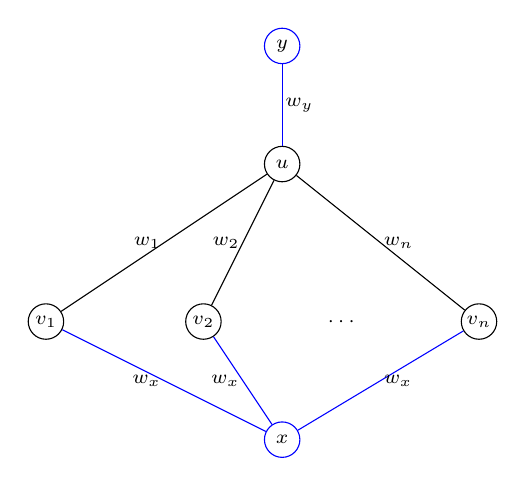
\begin{tikzpicture}[scale=1, every node/.style={inner sep=1pt}]
            \scriptsize
            % Nodes
            \node[draw, circle, minimum size=0.45cm] (u) at (0, 2) {$u$};
            \node[draw=blue, circle, minimum size=0.45cm] (y) at (0, 3.5) {$y$};
            \node[draw, circle, minimum size=0.45cm] (v1) at (-3, 0) {$v_1$};
            \node[draw, circle, minimum size=0.45cm] (v2) at (-1, 0) {$v_2$};
            \node[draw, circle, minimum size=0.45cm] (vn) at (2.5, 0) {$v_n$};
            \node[draw=blue, circle, minimum size=0.45cm] (x) at (0, -1.5) {$x$};

            % Connecting edges
            \draw (u) -- (v1) node[midway, left] {$w_1$};
            \draw (u) -- (v2) node[midway, left] {$w_2$};
            \draw (u) -- (vn) node[midway, right] {$w_n$};
            \draw[draw=blue] (u) -- (y) node[midway, right] {$w_y$};
            \draw[draw=blue] (v1) -- (x) node[midway, left] {$w_x$};
            \draw[draw=blue] (v2) -- (x) node[midway, left] {$w_x$};
            \draw[draw=blue] (vn) -- (x) node[midway, right] {$w_x$};

            % Dots
            \path (v2) -- (vn) node[midway, draw=none] {$\cdots$};
        \end{tikzpicture}
    \end{minipage}
    \hfill
    \begin{minipage}{0.48\textwidth}
        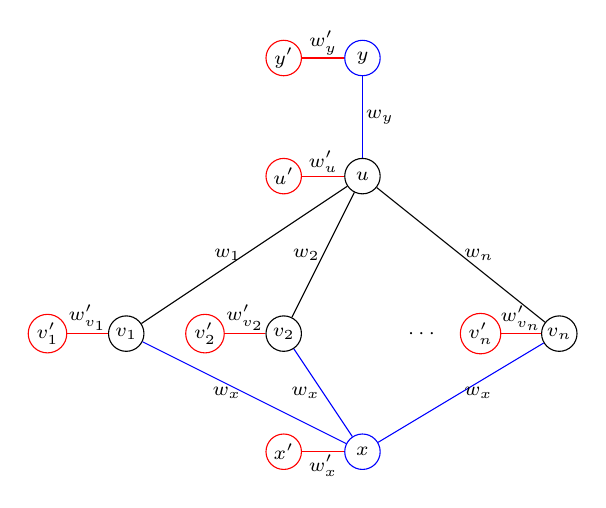
\begin{tikzpicture}[scale=1, every node/.style={inner sep=1pt}]
            \scriptsize
            % Nodes
            \node[draw, circle, minimum size=0.45cm] (u) at (0, 2) {$u$};
            \node[draw=blue, circle, minimum size=0.45cm] (y) at (0, 3.5) {$y$};
            \node[draw, circle, minimum size=0.45cm] (v1) at (-3, 0) {$v_1$};
            \node[draw, circle, minimum size=0.45cm] (v2) at (-1, 0) {$v_2$};
            \node[draw, circle, minimum size=0.45cm] (vn) at (2.5, 0) {$v_n$};
            \node[draw=blue, circle, minimum size=0.45cm] (x) at (0, -1.5) {$x$};

            \node[draw=red, circle, minimum size=0.45cm] (u') at (-1, 2) {$u'$};
            \node[draw=red, circle, minimum size=0.45cm] (y') at (-1, 3.5) {$y'$};
            \node[draw=red, circle, minimum size=0.45cm] (v'1) at (-4, 0) {$v'_1$};
            \node[draw=red, circle, minimum size=0.45cm] (v'2) at (-2, 0) {$v'_2$};
            \node[draw=red, circle, minimum size=0.45cm] (v'n) at (1.5, 0) {$v'_n$};
            \node[draw=red, circle, minimum size=0.45cm] (x') at (-1, -1.5) {$x'$};

            % Connecting edges
            \draw (u) -- (v1) node[midway, left] {$w_1$};
            \draw (u) -- (v2) node[midway, left] {$w_2$};
            \draw (u) -- (vn) node[midway, right] {$w_n$};
            \draw[draw=blue] (u) -- (y) node[midway, right] {$w_y$};
            \draw[draw=blue] (v1) -- (x) node[midway, left] {$w_x$};
            \draw[draw=blue] (v2) -- (x) node[midway, left] {$w_x$};
            \draw[draw=blue] (vn) -- (x) node[midway, right] {$w_x$};

            \draw[draw=red] (y) -- (y') node[midway, above] {$w'_y$};
            \draw[draw=red] (u) -- (u') node[midway, above] {$w'_u$};
            \draw[draw=red] (v1) -- (v'1) node[midway, above] {$w'_{v_1}$};
            \draw[draw=red] (v2) -- (v'2) node[midway, above] {$w'_{v_2}$};
            \draw[draw=red] (vn) -- (v'n) node[midway, above] {$w'_{v_n}$};
            \draw[draw=red] (x) -- (x') node[midway, below] {$w'_x$};

            % Dots
            \path (v2) -- (vn) node[midway, draw=none] {$\cdots$};
        \end{tikzpicture}
    \end{minipage}
    \caption{(Left) $G;\quad$(Right) We add partner vertices, shown in red, for every vertex in $G$ to get $G'$}
    \label{fig:extended_graph}
\end{figure}

    % \textbf{Construction:} \\
    % \todo[inline]{RG: Change $V$ to $U\cup V$.}
    We will construct $\{G',w',b'\}$ from $\{G,w,b\}$. Let $\nu$ and $\nu'$ represent the characteristic functions of the $b$-matching games in $G$ and $G'$ respectively.
    Construct the graph $G'=(U', V', E')$ from $G=(U, V, E)$ as follows. For every vertex $v$ in $U\cup V$, there are two vertices - $v, v'$ - in $U'\cup V'$. Call $v$'s as the \textit{original} vertices and $v'$'s, the \textit{partner} vertices of respective original vertex $v$.
    
    Preserve all the edges from $G$ in $G'$, i.e., if $(u,v)\in E$, then $(u,v)\in E'$. Weights of all such edges will remain the same. Add an edge between every vertex and its partner, i.e., $\forall v\in U\cup V, (v,v')\in E'$. The weights of these edges will be set based on the profits of agents in $p$ and weights of edges in $E$ as follows. Let $$p^* = 1+ \max{\{\max_{v\in U\cup V} p_v, \max_{e \in E} w_e \}}$$Then $$\forall v \in U\cup V,\quad w'_{(v,v')} = 2p^* - p_v$$ The capacities, $b':U'\cup V'\rightarrow \mathbb{Z}_+$ of all original vertices will be set one more than their capacities in $G$ and the capacities of partner vertices will be set to 1, i.e., $b'_v = 1 + b_v$ and $b'_{v'} = 1$.

    Note that $p^*$ is chosen so that for every vertex, the edge to its partner is heavier than all other edges incident on it - $$ w'_{(v,v')} = 2p^* - p_v = (p^* - p_v) + (p^*) > p^* > w_e,\forall {e \in E}$$ And since we have increased the capacities of all original vertices by 1 and set the capacities of all partner vertices to 1, this, in effect, ensures the following.

    \begin{claim}
    \label{cl:max_wt_b_matching}
        The max. wt. $b$-matching of $G'$ is some max. wt. $b$-matching in $G$ together with all edges between original vertices and their partners. 
    \end{claim}

    \begin{proof}
        Given any $b$-matching, not containing $(v,v')$ for some $v\in U\cup V$, we can include $(v,v')$, replacing any other edge incident on $v$ if necessary, to get another $b$-matching with a larger weight. Hence, every edge between an original vertex and its partner is chosen exactly once in the max. wt. $b$-matching in $G'$. Given these edges are chosen, the capacities on original vertices will become the same as in $G$, completing the proof.  
    \end{proof}

    Finally, consider the profit share $$\forall v\in U'\cup V', \quad p'(v) = p^*$$
    \begin{lemma}
        $p':U'\cup V'\rightarrow \mathbb{R}_+$ is an imputation in the $b$-matching game on $G'$.
    \end{lemma}

    \begin{proof}
        The total profit distributed by $p' = \sum_{v\in U'\cup V'} p^* = 2|(U'\cup V')|\cdot p^*$
        From \Cref{cl:max_wt_b_matching}, the total worth of the game is $\nu(G') = \nu(G)+\sum_{v\in U\cup V}(2p^*-p_v) = \nu(G) + 2|(U\cup V)|\cdot p^* - \sum_{v\in U\cup V} p_v$. Since $p:U\cup V\rightarrow \mathbb{R}_+$ is an imputation in $G$, $\sum_{v\in U\cup V} p_v = p(G) = \nu(G)$, and $\nu(G') = 2|U\cup V|\cdot p^* = p'(G')$. Hence, $p'$ is an imputation in the $b$-matching game on $G'$.
    \end{proof}

    Now we prove the main lemma. 

    \begin{lemma}
    \label{lem:leximin_reduction}
        $p'$ is not in the core of $(G',\nu')$ if and only if $p$ is not in the core of $(G,\nu)$.
    \end{lemma}

    \begin{proof}
        Assume $p$ is not in the core of $(G,\nu)$ as $p(S)<\nu(S)$ for some set $S\subseteq U\cup V$. Let $S'$ be the union of all original vertices and their partner vertices of every vertex in $S$. Then, like in the proof of \Cref{cl:max_wt_b_matching}, $$\nu'(S') = \nu(S) + \sum_{v\in S}(2p^*-p_v) = \nu(S) + 2|S|\cdot p^* - \sum_{v\in S}(p_v) = \nu(S) + 2|S|\cdot p^* - p(S)$$Also note that $p'(S') = 2|S|\cdot p^*$ as every vertex $v$ in $S'$ gets the same profit of $p^*$. Therefore $p(S) < \nu(S) \implies p'(S') < \nu'(S')$. This shows that if $p$ is not in the core of $(G,\nu)$ then $p'$ is not in the core of $(G',\nu')$.
        
    

        Now assume $p'$ is not in the core of $(G',\nu')$. Let $S^*\subseteq U'\cup V'$ be a \textit{minimal} set such that $p'(S^*)<\nu'(S^*)$. Note that, for every partner vertex $v'\in S^*$, $S^*$ must also contain the original vertex $v$. For otherwise, we can remove $v'$ from $S^*$ decreasing the profit but not the worth, contradicting the minimality of $S^*$.        
        
        Now, if $S^*$ contains an original vertex $v$ but not its partner $v'$, we can add $v'$ to $S^*$ and still maintain $p'(S^*\cup \{v'\})<\nu'(S^* \cup \{v'\})$ as this increases the value($2p^*-p_v$) more than the profit($p^*$). performing this operation for all original vertices, we will end up with a set $S'$ which has a vertex and its partners in pairs, and $p'(S') < \nu'(S')$.

        Now consider the sub-coalition of agents $S$ of just the original partner vertices in $S'$, in the game $(G,\nu)$. Note that, like above, $p'(S') = 2|S|\cdot p^*$ and $\nu'(S') = \nu(S) + \sum_{v\in S}(2p^*-p_v) = \nu(S) + 2|S|\cdot p^* - \sum_{v\in S}(p_v) = \nu(S) + 2|S|\cdot p^* - p(S)$.

        And so, if $p'(S') < \nu'(S')$ then $p(S) < \nu(S)$ proving the other direction of the lemma.
        
    \end{proof}

    Combining \Cref{lem:leximin_reduction} and \Cref{thm:core_coNP_complete}, we get that finding an unstable coalition in $(G',\nu')$ under imputation $p'$ is NP-hard. Since $p'$ is the imputation that distributes equal profit to all the agents, this proves that it is NP-hard to compute an imputation that maximizes the minimum profit or minimizes the maximum profit. 

\end{proof}

Since leximin and leximax imputations also maximize the minimum profit and minimize the maximum profit, it is also NP-hard to  compute them.

\begin{corollary}
\label{cor:leximin_NP_hard}
    Computing the leximin(or leximax) core imputation in a $b$-matching game is NP-hard.
\end{corollary}    

% \begin{theorem}
%     There's a pseudo-polynomial time algorithm to check if a profit share is in the core of $b$-matching games on general bipartite graphs graphs, with a constant number of vertices in one of the partitions.
% \end{theorem}

